
    \begin{abstract_online}{Molecular Dynamics Simulations on Interfacial Structure in Presence of Third Component}{%
        \underline{A. Das}$^{1, 3}$, Sk. M. Ali$^{2, 3}$}{%
        }{%
        $^1$ Nuclear Recycle Board, Bhabha Atomic Research Centre, Trombay, Mumbai, India\newline{}$^2$ Chemical Engineering Division, Bhabha Atomic Research Centre, Trombay, Mumbai, India\newline{}$^3$ Homi Bhabha National Institute, trombay, Mumbai, India}
    Microscopic understanding of the interface between two immiscible or partially miscible liquids for a biphasic system not only has an immense interest in view of mass transfer processes but also has significant technological importance in the field of science and engineering. Due to its inherent difficulty, the understanding of molecular details at liquid–liquid interface using only experimental technique is not enough to ascertain the interfacial behaviour mostly due to the fluidity of the interface and buried surroundings. The contribution of intrinsic thickness and broadening induced by capillary waves ($w_c$) are responsible for total thickness but their determination are perchance not encountered for three components system. In this context, we have performed molecular dynamics (MD) simulations of a technologically important water–dodecane system containing tri-isoamyl phosphate (TiAP) used for reprocessing of radionuclide. MD simulations provide a microscopic view of the interfacial properties of water–dodecane/TiAP interface. Further, an empirical relation between interfacial tension and interface thickness has been established for water–dodecane/TiAP system [1] (see inset of Fig. 1) which is also related by capillary wave theory (CWT) as: $$w_c^2 = \frac{k_B T}{2 \pi \gamma} ln \left( \frac{L_{II}}{L_b} \right)$$  Here, $k_B$ is Boltzmann constant and $T$ is temperature, $L_{II}$ is the box dimension along $x$ or $y$ direction. $L_b$ represents bulk correlation length commonly expressed in terms of molecular length which is evaluated from the volume determined by COSMOtherm program at the BP/TZVP level of theory as implemented in Turbomole package. The calculated $w_c$ for water–dodecane system [1] (0.202 nm) is in good agreement with reported $(0.338nm)$ results [2]. For a three components system, it is reasonable to introduce the weighted average of dodecane and TiAP for determination of Lb to account the effect of TiAP. Furthermore, the total interface thickness ($w_t$) cannot be solely represented by $w_c$. The wt can be empirically fitted as [1]: $$w_t^2 = \frac{(\sigma_{water} + \sigma_{TiAP} + \sigma_{dodecane})}{1.4 \sigma_{water}} \frac{k_B T}{\gamma} ln \left( \frac{L_{II}}{L_b} \right)$$  The total interface thickness obtained from density curve and Eq. (2) are in good agreement as shown in Fig. 1 as a function of mole fraction of TiAP and acid concentration.  Eq. (2) might be useful for determining $w_t$ for a wide range of bi-phasic system.  \begin{center}  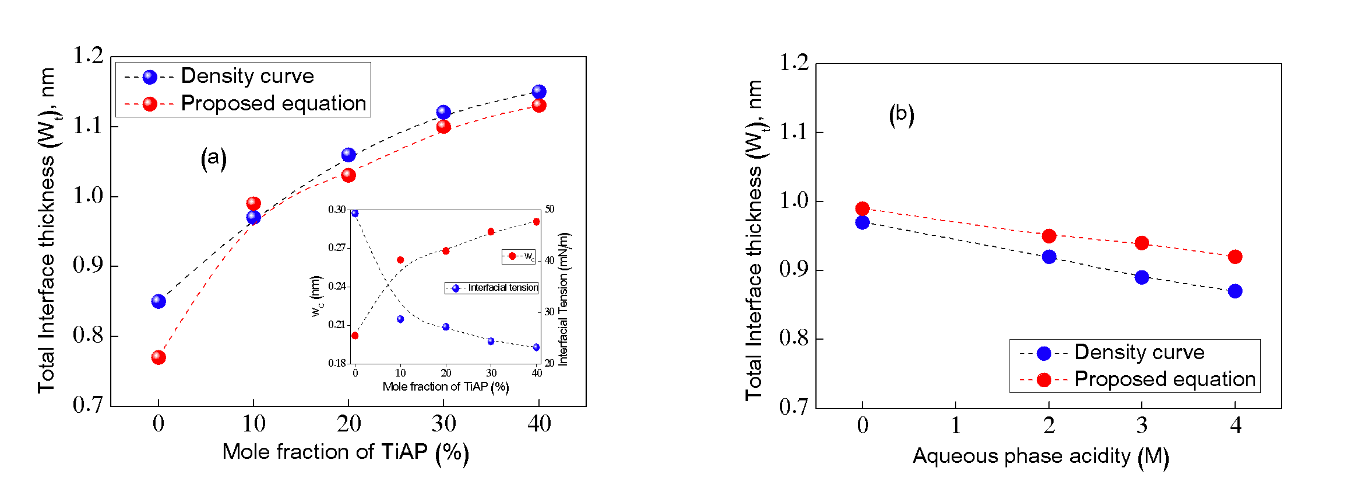
\includegraphics[width=\linewidth]{abstracts/txt/figures/arya_img.png}  \caption{$W_t$  from density curve and  Eq. (2) as a function of (a) mole fraction and (b) aqueous phase acidity. $W_c$  and  vs. mole fraction of TiAP [inset of Fig. (a)]}  \end{center}  
    
        \textbf{References} \newline{}[1] A. Das, Sk. M. Ali, J. Mol. Liq, 2019, 277, 217–232.\newline{}[2] D. M. Mitrinovic, A. M. Tikhonov, M. Li, Z. Huang and M. L. Schlossman, Phys. Rev. Lett. 2000, 85, 582.
    \end{abstract_online}
    